\documentclass[10pt]{beamer}

\usepackage{polyglossia}
\usepackage{csquotes}
\usepackage{fontspec}
\usepackage{microtype}
\usepackage{color}
\usepackage{url}
\usepackage{hyperref}
\usepackage{amsfonts}
\usepackage{amsthm}
\usepackage{amsmath}

\setdefaultlanguage{english}
\setmainfont{TeX Gyre Termes}
\usetheme{Boadilla}
\usecolortheme{crane}
\setbeamertemplate{section in toc}[ball unnumbered]
\setbeamertemplate{bibliography item}{}

\hypersetup{
	pdfencoding=auto,
	unicode=true,
	citecolor=green,
	filecolor=blue,
	linkcolor=red,
	urlcolor=blue
}

\makeatletter
\newcommand*{\currentSection}{\@currentlabelname}
\makeatother

\title[Learning a metric for clustering structured data]
{
	Learning a metric for clustering structured data
}

\titlegraphic
{
	
\includegraphics[width=0.2\columnwidth]{images/cisco.png}
}

\author[Marek Dědič]
{
	Marek~Dědič\inst{1}\inst{2} \\
}

\institute[FJFI ČVUT v Praze]
{
	\inst{1} ČVUT v Praze, Fakulta jaderná a fyzikálně inženýrská, Matematická informatika \and
	\inst{2} Cisco Systems Inc., Karlovo náměstí 10, Praha 2
}

\AtBeginSection[]{
	\begin{frame}{\currentSection}
		\tableofcontents[currentsection]
	\end{frame}
}

\begin{document}

\begin{frame}
	\titlepage
\end{frame}

\begin{frame}{Obsah}
	\tableofcontents
\end{frame}

% Body

\section{Motivation}

\begin{frame}{Motivation}
	\begin{itemize}
		\item Enable clustering of IPs from SwFlows - enhance Correlation
		\item Take advantage of the structure of the data using MIL
		\item Try out unsupervised learning
	\end{itemize}
\end{frame}

\section{MIL}

\begin{frame}
	\centering
	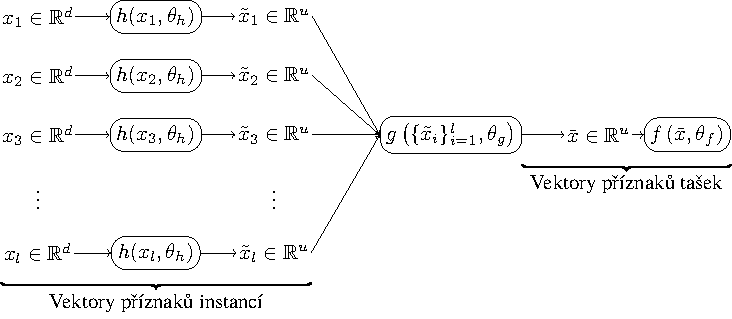
\includegraphics[width=0.9\pagewidth]{images/embedding_function/embedding_function.pdf}
\end{frame}

\section{Contrastive predictive coding}

\begin{frame}{Contrastive predictive coding}
	The ideas of contrastive predictive coding were originally adapted giving a loss function
	\[ \log \left\lVert f \left( B_n^{(1)} \right) - f \left( B_n^{(2)} \right) \right\rVert^2 - \log \sum_{j = 1}^K \left\lVert f \left( B_n^{(1)} \right) - f \left( B'_j \right) \right\rVert^2 \]
\end{frame}

\begin{frame}{Contrastive predictive coding}
	Later on, the loss function was simplified to
	\[ D_{ij} = \left\lVert f \left( B_i^{(1)} \right) - f \left( B_j^{(2)} \right) \right\rVert_2^2 \]
	\[ \frac{1}{n} \sum_{i = 1}^n \left( \log \left( D_{ii} \right) - \log \left( \sum_{i \neq j} D_{ij} \right) \right) \]
\end{frame}

\begin{frame}{Contrastive predictive coding - preliminary results (Musk)}
	\centering
	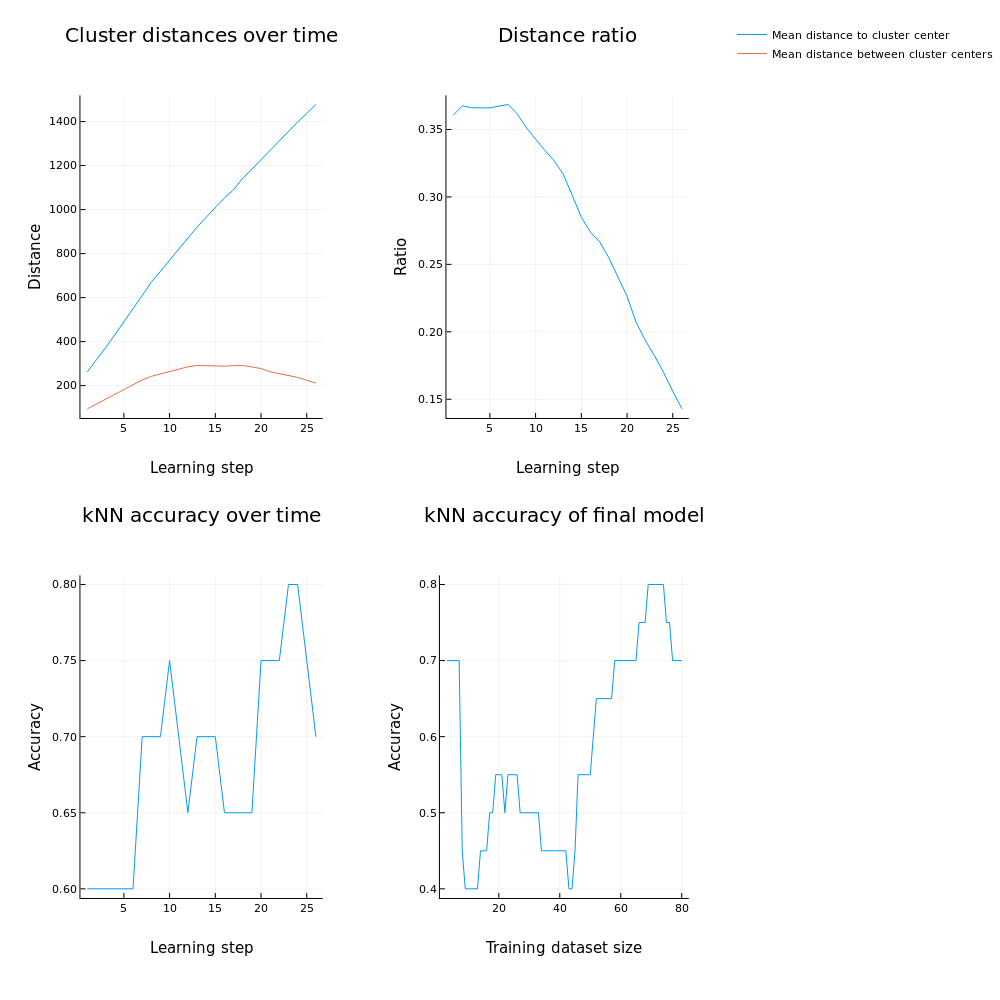
\includegraphics[width=0.7\pagewidth]{images/CPC.png}
\end{frame}

\section{Triplet loss}

\begin{frame}{Triplet loss}
	The triplet loss is another alternative, this time requiring supervised learning
	\[ y_{ij} =
\begin{cases}
	1 &\text{for} \quad y_i = y_j \\
	0 &\text{otherwise}
\end{cases}
\]
\[ \sum_{ij} y_{ij} D_{ij} + c \sum_{ijl} y_{ij} \left( 1 - y_{il} \right) \max \left( 0, 1 + D_{ij} - D_{il} \right) \]
\end{frame}

\begin{frame}{Triplet loss - preliminary results (Musk)}
	\centering
	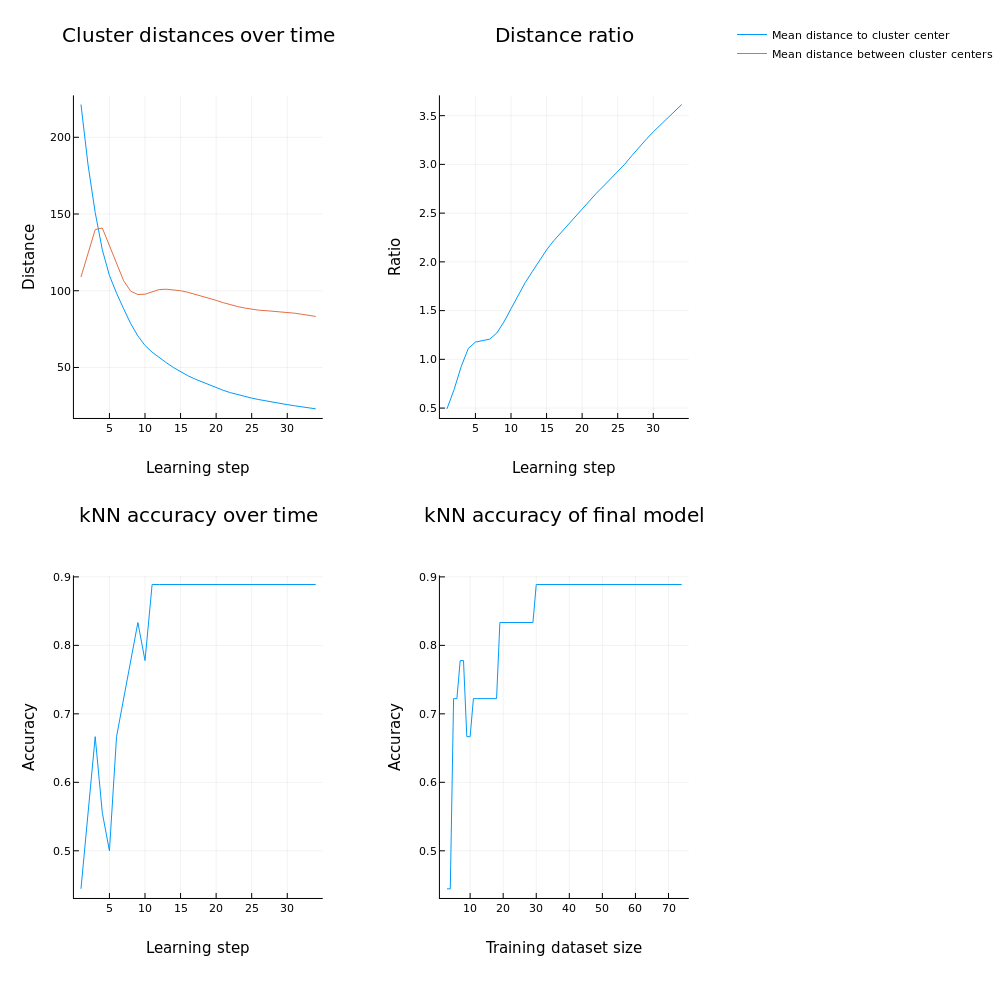
\includegraphics[width=0.7\pagewidth]{images/triplet.png}
\end{frame}

\end{document}
